% ======================================================================
% Master Manuscript — Part I (Reader's Guide) + Part II (Analytic Core) + Part III (Structural Corollaries)
% ======================================================================

\documentclass[11pt]{article}

% ------------------ Basic packages (minimal) ------------------
\usepackage[a4paper,margin=1in]{geometry}
\usepackage{amsmath,amssymb,amsthm,mathtools}
\usepackage{microtype}
\usepackage{hyperref}
\usepackage{tabularx,booktabs,array}
\usepackage{enumitem}
\usepackage{needspace}
\usepackage{caption}
\usepackage{float}

% >>> NEW: for long tables and in-document plotting of the error-vs-cutoff curve
\usepackage{longtable}
\usepackage{pgfplots}
\pgfplotsset{compat=1.18}

% ------------------ Theorem styles ------------------
\numberwithin{equation}{section}
\newtheorem{theorem}{Theorem}[section]
\newtheorem{lemma}[theorem]{Lemma}
\newtheorem{proposition}[theorem]{Proposition}
\newtheorem{corollary}[theorem]{Corollary}
\theoremstyle{remark}
\newtheorem{remark}[theorem]{Remark}

% ------------------ Col types ------------------
\newcolumntype{L}{>{\raggedright\arraybackslash}X}

% ------------------ Macros: frames, functions, projectors ------------------
\newcommand{\C}{\mathbb{C}}
\newcommand{\R}{\mathbb{R}}
\newcommand{\Z}{\mathbb{Z}}
\newcommand{\D}{\mathbb{D}}
\newcommand{\Real}{\operatorname{Re}}
\newcommand{\Imag}{\operatorname{Im}}
\newcommand{\zetaTwo}{\zeta_2}
\newcommand{\LambdaTwo}{\Lambda_2}
\newcommand{\LamTwo}{\LambdaTwo}
\newcommand{\Afac}{A_2}
\newcommand{\chiTwo}{\chi_2}
\newcommand{\Podd}{P_{\mathrm{odd}}}
\newcommand{\Peven}{P_{\mathrm{even}}}
\newcommand{\Ucore}{U}
\newcommand{\UR}{U_{\mathrm{R}}}
\newcommand{\UL}{U_{\mathrm{L}}}
\newcommand{\Ecomp}{E}
\newcommand{\Gout}{G_{\mathrm{out}}}
\newcommand{\Zloc}{Z_{\mathrm{loc}}}
\newcommand{\Arg}{\operatorname{Arg}}
\newcommand{\sgn}{\operatorname{sgn}}
\newcommand{\ii}{\mathrm{i}}

\newenvironment{Overview}{\begin{quote}\itshape}{\end{quote}}

% ------------------ Title page ------------------
\title{\Large A Height--Local Width--2 Program for Excluding Off--Axis Quartets\\[2pt]
\large with an Analytic Tail and a Rigorous Certified Criterion}
\author{Dylan Anthony Dupont}
\date{\today}

\begin{document}
\maketitle

\begin{abstract}
\noindent
The paper is organized in three parts:\;
\textbf{Part~I} (Reader’s Guide) reduces RH to a height--local target \(a(m)=0\) in the width--2 frame and records non--load--bearing scaffolding;\;
\textbf{Part~II} gives a self--contained, boundary--only analytic proof that at each nontrivial height the tilt vanishes \(a(m)=0\) via a disc--based \(L^2\) upper envelope and an \(L^2\) lower envelope (allocation + restricted contour + Jensen), plus an optional certified Outer/Rouch\'e path;\;
\textbf{Part~III} promotes the toolbox identities to structural corollaries and presents a deterministic, prime--locked generator of the ordinates.
\end{abstract}

\tableofcontents

% ======================================================================
% Part I — Reader’s Guide / Motivation, Reduction & Implications
% ======================================================================
\section*{Part I --- Reader’s Guide / Motivation, Reduction \& Implications}
\addcontentsline{toc}{section}{Part I --- Reader’s Guide / Motivation, Reduction \& Implications}

\paragraph{What this section is (and is not).}
\emph{What it does.} It introduces modulated frames and the width--2 normalization, defines the centered “\(a\)--lens” that measures horizontal tilt at a fixed height, and reduces RH to the height--local target \(a(m)=0\) for each nontrivial height \(m\). It also records a structural toolbox (projectors, rectifier, canonical stream, recurrence, curvature extractor, seed$\to$rectifier) and explains how these become \emph{corollaries} after Part~II.

\noindent\emph{What it does not do.} It contains no analytic estimates and no proofs. The hinge--unitarity fact and all bounds are proved later. This Guide is not used by the analytic part.

\subsection*{1) Modulated frames and the width--2 pivot}
For \(f>0\) define the modulated family \(\zeta_f(s):=\zeta(s/f)\) with completed form
\[
\Lambda_f(s)=\pi^{-\,s/(2f)}\,\Gamma\!\Big(\frac{s}{2f}\Big)\,\zeta_f(s),
\]
so \(\Lambda_f\) is entire and satisfies \(\Lambda_f(s)=\Lambda_f(f-s)\). Equivalently, \(\zeta_f(s)=A_f(s)\,\zeta_f(f-s)\) with \(A_f(s)A_f(f-s)\equiv1\).

\smallskip
\noindent\textbf{Width--2 normalization.} Put \(u:=(2/f)\,s\). Then
\[
\zetaTwo(u):=\zeta(u/2),\qquad
\LambdaTwo(u):=\pi^{-u/4}\Gamma(u/4)\,\zeta(u/2),\qquad
\LambdaTwo(u)=\LambdaTwo(2-u).
\]
The non--completed FE reads \(\zetaTwo(u)=\Afac(u)\,\zetaTwo(2-u)\).
In the open strip \(0<\Real u<2\) and \(\Imag u\neq0\), \(\Afac\) is analytic and nonvanishing.

\smallskip
\noindent\textbf{Partner map.} On \(\Imag u>0\), FE + conjugation gives the involution \(J(u)=2-\overline{u}\), swapping the two column points at the same height.

\smallskip
\noindent\textbf{Hinge unitarity (deferred).} The statement “\(|\chiTwo(u)|=|\Afac(u)|^{-1}=1\)” iff \(\Real u=1\) is proved in Part~II (Hinge--Unitarity, Theorem~\ref{thm:hinge}; see also Appendix~\ref{app:hinge-short}).

\subsection*{2) Centered \(a\)--lens and the quartet}
Let \(v:=u-1\) and \, \(E(v):=\LambdaTwo(1+v)\). Then \(E(v)=E(-v)=\overline{E(\overline v)}\).
A “nontrivial height” \(m>0\) means \(m\) occurs as the imaginary part of a nontrivial zero \(s=\tfrac12+\ii m/2\).
At fixed \(m>0\), set
\[
\UR(m;a)=1+a+\ii m,\qquad \UL(m;a)=1-a+\ii m,\qquad a\in[0,1).
\]
In the centered frame, the dial points are \(\pm(a+\ii m)\); the partner map \(J\) swaps \(\UR\leftrightarrow \UL\).
Conjugation plus FE reflection generate the quartet \(\{\,1\pm a\pm \ii m\,\}\).

\subsection*{3) Why width--2: slope invariance}
If the columns collapse at height \(m\) (\(a=0\)), the point is \(u=1+\ii m\) and its slope is \(\Imag u/\Real u = m\).
Rescaling to any frame \(s=(f/2)\,u\) preserves slope:
\[
\frac{\Imag s}{\Real s}=\frac{(f/2)\,m}{f/2}=m.
\]

\subsection*{4) Height--local reduction of RH}
Fix \(m>0\) and write \(\UR=1+a+\ii m\), \(\UL=1-a+\ii m\). The following equivalent algebraic forms are used:
\begin{itemize}[leftmargin=1.2em]
  \item (PHU--1) \(\Real \UR=\Real \UL \iff a=0\).
  \item (PHU--2) \(\Imag \UR/\Real \UR=\Imag \UL/\Real \UL \iff a=0\).
  \item (PHU--3) \(\UR=\UL=1+\ii m\).
\end{itemize}
Thus \(\mathrm{RH}\iff\) for every nontrivial height \(m>0\), \(a(m)=0\).

\subsection*{5) Box alignment and hand--off (no circularity)}
For later reference, define
\[
B(\alpha,m,\delta)=[\alpha-\delta,\alpha+\delta]\times[m-\delta,m+\delta],\qquad
\delta:=\eta\,\alpha/(\log m)^2,\ \ \eta\in(0,1).
\]
When \(\alpha=\pm a\), the dials \(\pm(a+\ii m)\) lie on the horizontal centerline.
\emph{What Part~II does.} Using only boundary analysis on such boxes (completed FE symmetry, Cauchy--Riemann transport, three--lines tools, Stirling--class envelopes, explicit control of \(\zeta'/\zeta\) away from zeros), Part~II shows any off--axis quartet forces a boundary lower bound larger than an explicit upper bound, hence \(a(m)=0\).

\subsection*{6) Parity gating and selection devices (interpretive only)}
In width--2,
\[
\zetaTwo(u)=\Afac(u)\,\zetaTwo(2-u),\quad
\Afac(u)=2^{u/2}\,\pi^{\,u/2-1}\,\sin\!\Big(\frac{\pi u}{4}\Big)\,\Gamma\!\Big(1-\frac{u}{2}\Big).
\]
On \(0<\Real u<2\), \(\Imag u\neq0\), the prefactor \(\Afac(u)\) is nonzero; its sine zeros lie on the real axis only. Thus \emph{inside} the open strip only \(\zetaTwo\) can vanish (nontrivial), while the trivial ladder is confined to \(\Real u\). This motivates an odd/even split on the integer lattice via
\[
\Podd(n)=\tfrac{1-\cos(\pi n)}{2},\qquad
\Peven(n)=\tfrac{1+\cos(\pi n)}{2}.
\]
We assign the nontrivial stream to odd slots and the trivial ladder to even slots. (Interpretive; not used in Part~II.)

\subsection*{7) Toolbox \(\to\) structural consequences (after the theorem)}
The items (columns/templates, canonical stream, single–frequency collapse, self–indexed recurrence, curvature extractor, seed\(\to\)rectifier) become \emph{Structural Corollaries in Part~III} once Part~II proves \(a(m)=0\). No toolbox component is used as an input in Part~II.

% ======================================================================
% Part II — Analytic Core (self-contained; boundary-only)
% ======================================================================
\section*{Part II --- Self-Contained Boundary--Only Contradiction on Aligned Boxes}
\addcontentsline{toc}{section}{Part II --- Self-Contained Boundary--Only Contradiction on Aligned Boxes}

In the width‑2 centered frame \(u=2s\), \(v=u-1\), let \(\LamTwo(u)=\pi^{-u/4}\Gamma(u/4)\zeta(u/2)\) and \(E(v)=\LamTwo(1+v)\).
We present a boundary‑only, height‑local program to exclude off‑axis quartets \(\{\pm a\pm i m\}\) via two complementary routes:
\begin{enumerate}[label=(\arabic*)]
\item an \emph{analytic tail}, uniform in \(\alpha\in(0,1]\), using only: (i) explicit short‑side forcing \(\ge \pi/2\); (ii) a residual bound for \(F=E/\Zloc\) with perimeter factor \(8\delta\); (iii) a disc‑based, \(L^2\) boundary‑to‑midpoint estimate with \emph{shape‑only} constants;
\item a rigorous \emph{Outer/Rouch\'e Certification Path} (optional): interval arithmetic on \(\partial B\) + validated Poisson + Lipschitz grid\(\to\)continuum enclosure \(\Rightarrow \sup_{\partial B}\!\big|E-\Gout\big|/|\Gout|<1\Rightarrow\) zero‑free box, followed by Bridge~1 (inner collapse \(W\equiv e^{i\theta}\)) and Bridge~2 (stitching).
\end{enumerate}
We also prove a corner outer interpolation from continuous Dirichlet data.
All constants in the upper/lower envelope are \emph{shape‑only} (independent of \(m,\alpha,a\)); residual constants are symbolic and optionally instantiated in Appendix~\ref{app:S2-nums}. %% [PATCH P1]

% ---------------------------------------------------
\Needspace{16\baselineskip}
\section*{Symbols \& Provenance (at a glance)}
\addcontentsline{toc}{section}{Symbols \& Provenance (at a glance)}

\small
\begin{center}
\begin{tabularx}{\textwidth}{@{}p{3.8cm} L L@{}}
\toprule
\textbf{Symbol} & \textbf{Definition / role} & \textbf{Provenance / rationale}\\
\midrule
$u=2s$, $v=u-1$ & Width--2 frame centered at $\Real u=1$ & Centers functional equation symmetry\\
\midrule
$\LamTwo(u)=\pi^{-u/4}\Gamma(u/4)\zeta(u/2)$ & Completed object & Standard; FE for $\LamTwo$; width--2 transport\\
\midrule
$E(v)=\LamTwo(1+v)$ & Workhorse in $v$--plane & Even \& conjugate symmetrical: $E(v)=E(-v)=\overline{E(\bar v)}$\\
\midrule
$\zeta_2(u)=\zeta(u/2)$ & Width--2 zeta & Used in FE and hinge law\\
\midrule
$\chiTwo(u)$ & FE factor inverse & $\chiTwo(u)=\pi^{u/2-1/2}\frac{\Gamma((2-u)/4)}{\Gamma(u/4)}$\\
\midrule
$B(\alpha,m,\delta)$ & $[\alpha-\delta,\alpha+\delta]\times[m-\delta,m+\delta]$ & Square centered at $(\alpha,m)$, side $2\delta$\\
\midrule
$\alpha\in(0,1]$ & Horizontal center & Worst case $\alpha=1$; left dial via reflection $w=-v$\\
\midrule
$m\ge 10$ & Height parameter & Ensures uniform DLMF/Titchmarsh/Ivi\'c regimes\\
\midrule
$\delta=\dfrac{\eta\,\alpha}{(\log m)^2}$, $\eta\in(0,1)$ & Half--side length of $B$ & Balances forcing vs.\ residual $O(\delta\log m)$\\
\midrule
$\partial B$, $I_\pm$, $Q$ & Boundary, short verticals, horizontals & Boundary integrals/suprema; quiet arcs\\
\midrule
$\Zloc(v)=\prod_{|\Imag\rho-m|\le 1}(v-\rho)^{m_\rho}$ & Local zero/pole factors & De--singularizes $E$ near $\partial B$\\
\midrule
$F=E/\Zloc$ & Residual analytic factor & Lemma~\ref{lem:residual} (constants symbolic)\\
\midrule
$G(v)=\dfrac{E(1+v)}{E(1-v)}$ & Odd--lane quotient & Links to hinge; two--point identity\\
\midrule
$\Gout=e^{U+iV}$ & Modulus--outer with $|\Gout|=|E|$ on $\partial B$ & $U=\log|E|$ solves Dirichlet; $V$ harmonic conjugate\\
\midrule
$W=E/\Gout$ & Inner quotient ($|W|=1$ a.e.\ on $\partial B$) & Collapses to unimodular constant upon certification\\
\midrule
$v_\pm^\star=\pm(a+im)$ & Dial pair & Points of evaluation in the tail on centerline\\
\midrule
$Z_{\rm pair}(v)$ & $(v-(a+im))(v-(-a+im))$ & Short--side forcing on $I_+$\\
\midrule
$\Gamma_\lambda$ & Central $\lambda\delta$ sub--arcs + tiny joins & Restricted contour (zero forcing)\\
\midrule
$B_{\rm core}(a,m;\lambda)$ & Dial--centred core box & Zero location forced by $\Gamma_\lambda$\\
\midrule
$K_{\rm alloc}^{(\star)}(\lambda)$ & Allocation coefficient & Shape--only; Lemma~\ref{lem:allocL2}\\
\midrule
$c_0=\tfrac{1}{4\pi}\log(2\sqrt{2})$ & Dial deficit constant ($\lambda=\tfrac12$) & From Jensen at dial; Lemma~\ref{lem:jensen-dial}\\
\midrule
$C_{\mathrm{up}}$ & Upper--envelope constant & Disc--based bound; Lemma~\ref{lem:upper-disc}\\
\midrule
$C_h''$ & Horizontal budget constant & Shape--only; Lemma~\ref{lem:corezero}\\
\bottomrule
\end{tabularx}
\end{center}
\normalsize

\medskip
\noindent\textit{Sources.} Digamma: DLMF §5.5 (reflection), §5.11 (vertical--strip bounds). $\zeta'/\zeta$: Titchmarsh, \textit{The Theory of the Riemann Zeta-Function}, §14; Ivi\'c, \textit{The Riemann Zeta-Function}, Ch.~9. Lipschitz Hilbert/Cauchy and boundary traces: Coifman--McIntosh--Meyer (1982); Duren; Garnett.

% ---------------------------------------------------
\section{Frames, symmetry, and the hinge law}\label{sec:frames}
% ---------------------------------------------------

We work in the width--2 centered frame \(u=2s\), \(v=u-1\), with
\[
\LamTwo(u)=\pi^{-u/4}\Gamma\!\Big(\frac{u}{4}\Big)\zeta\!\Big(\frac{u}{2}\Big),\qquad
E(v):=\LamTwo(1+v).
\]
Then \(E(v)=E(-v)=\overline{E(\bar v)}\) and off‑axis zeros appear as quartets \(\{\pm a\pm im\}\) by the FE symmetry plus conjugation.

\begin{theorem}[Hinge--Unitarity]\label{thm:hinge}
Let \(\zeta_2(u)=\zeta(u/2)\) and \(\zeta_2(u)=A_2(u)\,\zeta_2(2-u)\) with
\[
\chiTwo(u):=A_2(u)^{-1}=\pi^{u/2-1/2}\frac{\Gamma\big(\frac{2-u}{4}\big)}{\Gamma\big(\frac{u}{4}\big)}.
\]
For each fixed \(t\neq 0\), define \(f(\sigma)=\log|\chi_2(\sigma+it)|\). Then
\[
f'(\sigma)=\tfrac12\log\pi-\tfrac12\,\Real\psi\!\Big(\tfrac{\sigma+it}{4}\Big)
-\tfrac14\,\Real\!\Big[\pi\cot\!\Big(\tfrac{\pi}{4}(\sigma+it)\Big)\Big].
\]
Moreover,
\[
\big|\Real\!\big[\pi\cot(x+iy)\big]\big|\le\frac{\pi}{\cosh(2y)-1}.
\]
With \(x=\tfrac{\pi}{4}\sigma\), \(y=\tfrac{\pi}{4}|t|\), for \(|t|\ge m_1/2\) (Appendix~\ref{app:firstheight-certified}) the cotangent term is negligible, and vertical‑strip bounds give
\(\Real\psi\!\big(\frac{\sigma+it}{4}\big)\ge \log\!\big(\frac{|t|}{4}\big)-\frac{2}{|t|}\).
Hence \(f'(\sigma)<0\) on \(\R\) for such \(t\). Since \(f(1)=0\), we have \(|\chi_2(u)|=1\) iff \(\Real u=1\).
A short proof is also recorded in Appendix~\ref{app:hinge-short}.
\end{theorem}

% ---------------------------------------------------
\section{Boxes, de-singularization, residual control, and forcing}\label{sec:boxes}
% ---------------------------------------------------

Fix \(m\ge 10\), \(\alpha\in(0,1]\), and
\begin{equation}\label{eq:box-delta}
B(\alpha,m,\delta)=\big[\alpha-\delta,\alpha+\delta\big]\times\big[m-\delta,m+\delta\big],
\qquad
\delta=\frac{\eta\,\alpha}{(\log m)^2},\ \ \eta\in(0,1).
\end{equation}

\begin{lemma}[Short boxes stay in \(\Real v>0\)]\label{lem:box-right}
For \(m\ge10\) and any \(\eta\in(0,1)\), one has \(\delta<\alpha\) and \(B(\alpha,m,\delta)\subset\{\Real v>0\}\), uniformly in \(\alpha\in(0,1]\).
\end{lemma}
\begin{proof}
Since \(\eta/(\log m)^2<1\), we have \(\delta=\alpha\,\eta/(\log m)^2<\alpha\), so the left edge is \(\alpha-\delta>0\).
\end{proof}

\paragraph{De--singularization on \(\partial B\).}
Let
\begin{equation}\label{eq:Zloc}
\Zloc(v)=\prod_{\rho:\,|\Imag\rho-m|\le 1}(v-\rho)^{m_\rho},\qquad
F(v):=\frac{E(v)}{\Zloc(v)}.
\end{equation}
Then \(F\) is analytic and zero‑free on a neighborhood of \(\partial B\) (all local zeros/poles with \(|\Imag\rho-m|\le 1\) have been removed).
If a zero/pole meets \(\partial B\), shrink \(\delta\) by \(1-\varepsilon\) or shift \(\alpha\) by \(O(\delta)\); all bounds below are stable under \(O(\delta)\) changes.

\begin{lemma}[Residual envelope]\label{lem:residual}
On \(\partial B\),
\begin{equation}\label{eq:residual-sup}
\sup_{\partial B}\Big|\frac{F'}{F}\Big|\ \le\ C_1\log m + C_2,
\end{equation}
and
\begin{equation}\label{eq:residual-perimeter}
\big|\Delta_{\partial B}\arg F\big|\ \le\ 8\delta\,\big(C_1\log m+C_2\big).
\end{equation}
\emph{Justification.} DLMF §5.11 controls \(\psi\) on vertical strips; Titchmarsh §14 and Ivi\'c Ch.~9 control \(\zeta'/\zeta\) on \(1/2\le\sigma\le 1,\ t\ge 3\). After removing local poles via \eqref{eq:Zloc} and transporting to width–2, we obtain \eqref{eq:residual-sup}. For \eqref{eq:residual-perimeter}, write \(\Delta_{\partial B}\arg F=\int_{\partial B}\partial_\tau\arg F\,ds\) and bound by \(8\delta\,\sup|F'/F|\). We keep \(C_1,C_2>0\) symbolic (optional instantiation in Appendix~\ref{app:S2-nums}). %% [PATCH P2]
\end{lemma}

\begin{lemma}[Logarithmic derivatives on \(\partial B\)]\label{lem:bridge-logs}
On \(\partial B\),
\[
\frac{E'}{E}=\frac{F'}{F}+\frac{(Z_{\rm loc})'}{Z_{\rm loc}},\qquad
\sup_{\partial B}\Big|\frac{E'}{E}\Big|
\ \le\ \sup_{\partial B}\Big|\frac{F'}{F}\Big|+\sum_{\rho:\,|\Imag\rho-m|\le 1}\ \sup_{v\in\partial B}\frac{m_\rho}{|v-\rho|}\,.
\]
\end{lemma}

\begin{lemma}[Short--side forcing]\label{lem:short-side}
Let \(Z_{\rm pair}(v)=(v-(a+im))(v-(-a+im))\). On the near vertical
\[
I_+=\{\alpha+i y:\ |y-m|\le \delta\},\quad\text{with }|\alpha-a|\le\delta,
\]
one has
\begin{equation}\label{eq:short-side}
\Delta_{I_+}\arg Z_{\rm pair}
=2\arctan\frac{\delta}{|\alpha-a|}+2\arctan\frac{\delta}{\alpha+a}\ \ge\ \frac{\pi}{2}.
\end{equation}
\end{lemma}

% ---------------------------------------------------
\section{Boundary-only criteria, bridges, and corner interpolation}\label{sec:criteria}
% ---------------------------------------------------

\subsection{Two-point Schur/outer criterion (boundary-only)}\label{subsec:schur-criterion}

Let \(\varphi:\D\to B\) be conformal with \(\varphi(0)\) the box center and boundary map avoiding corners at two marked points. Define
\begin{equation}\label{eq:schur-def}
G(v):=\frac{E(1+v)}{E(1-v)},\qquad \Phi:=(G/H)\circ\varphi,
\end{equation}
where \(H\) is an outer majorant for \(G\) on \(B\): choose \(M\in C(\partial B)\) with \(M\ge |G|\) a.e.\ on \(\partial B\), let \(U\) solve the Dirichlet problem on \(B\) with boundary data \(\log M\), fix a harmonic conjugate \(V\), and set \(H=e^{U+iV}\). Then \(\Phi\in H^\infty(\D)\) with \(\|\Phi\|_\infty\le 1\) (Duren~\cite[§II.5]{DurenHp}; Garnett~\cite[§II.2]{GarnettBAF}).

\begin{proposition}[Two-point Schur pinning]\label{prop:schur-pin}
Under the setup above, suppose two non‑corner boundary points \(\zeta_\pm\in\partial\D\) have nontangential limits with \(|\Phi(\zeta_\pm)|=1\), and some boundary arc \(A\subset\partial\D\) has \(\operatorname*{ess\,sup}_{A}|\Phi|\le 1-\varepsilon\) with \(\varepsilon>0\). Then for any \(z\in\D\) with harmonic measure \(\omega_z(A)\ge\omega_*>0\),
\(|\Phi(z)|\le 1-\kappa\) with \(\kappa=\kappa(\varepsilon,\omega_*)>0\). Consequently, for \(v=\varphi(z)\): \(|G(v)|\le (1-\kappa)|H(v)|\).
\end{proposition}

\begin{lemma}[Two-point link for \(|G|\) and \(|\chi_2|\)]\label{lem:G-chi-link}
For \(v=a+im\),
\begin{equation}\label{eq:G-chi-product}
|G(a+im)|\,|G(-a+im)|
=\big|\chi_2(1+a+im)\big|\,\big|\chi_2(1-a+im)\big|.
\end{equation}
\emph{Derivation:} expanding \(\Lambda_2\) at \(1\pm v\) yields the identity; poles at \(v=0\) (the pole of \(\zeta\) at \(1\)) are avoided by the boundary‑contact convention. %% [PATCH P4]
\end{lemma}

\subsection{Outer/Rouch\'e Certification Path}\label{subsec:rouche-criterion}

Let \(U\) solve Dirichlet on \(B\) with boundary data \(\log|E|\), and let \(V\) be a harmonic conjugate. Set \(\Gout:=e^{U+iV}\).
Then \(\Gout\) is analytic and zero‑free on \(B\) with \(|\Gout|=|E|\) a.e.\ on \(\partial B\).

\begin{proposition}[Outer/Rouch\'e criterion]\label{prop:rouche-criterion}
If
\begin{equation}\label{eq:rouche-ratio}
\sup_{v\in\partial B}\frac{|E(v)-\Gout(v)|}{|\Gout(v)|}\ <\ 1,
\end{equation}
then \(E\) is zero‑free in \(B\) (Rouch\'e). Consequently, the inner quotient \(W:=E/\Gout\) is analytic and nonvanishing on \(B\) with \(|W|=1\) a.e.\ on \(\partial B\).
\end{proposition}

\begin{proposition}[Bridge~1: inner collapse]\label{prop:bridge1}
Under \eqref{eq:rouche-ratio}, \(\log|W|\) is harmonic with zero boundary trace on \(B\), hence \(|W|\equiv 1\) on \(B\). By the open mapping theorem, \(W\equiv e^{i\theta_B}\) on \(B\).
\end{proposition}

\begin{proposition}[Bridge~2: stitching]\label{prop:bridge2}
If \(B_1,B_2$ overlap and \(W\equiv e^{i\theta_{B_j}}\) on \(B_j$ \((j=1,2)\), then \(e^{i\theta_{B_1}}=e^{i\theta_{B_2}}\) on \(B_1\cap B_2\).
\end{proposition}

\begin{remark}[Certification recipe and reproducibility]
The verification of \eqref{eq:rouche-ratio} is performed by a rigorous pipeline detailed in Appendix~\ref{app:cert}.
\end{remark}

% ===================================================
\section{Analytic tail (uniform in \texorpdfstring{$\alpha$}{alpha})}\label{sec:tail}
% ===================================================

\paragraph{Setup.}
Let \(\varphi:\D\to B(\alpha,m,\delta)\) be conformal with \(\varphi(0)=\alpha+im\); define the dial pair \(v_\pm^\star=\pm(a+im)\) on the horizontal centerline. Split \(\partial B\) into the two \emph{quiet arcs} \(Q\) (horizontal edges) and the two short verticals \(I_\pm\). Write \(W:=E/\Gout\). We use \(\partial_\tau\) for unit tangential derivatives and \(ds\) for arclength; \(|\partial B|=8\delta\).
For the left dial \( -a+im\) we use reflection \(w=-v\); all shape‑only constants are unaffected.

\subsection{Upper envelope via a disc-based \(L^2\) route}\label{subsec:upper}

\begin{lemma}[Boundary phase \(\Rightarrow\) dial deficit; disc-based upper bound]\label{lem:upper-disc}
Let \(m\ge 10\) and \(\delta=\eta\,\alpha/(\log m)^2\). Let \(W=E/\Gout\) be analytic on \(B(\alpha,m,\delta)\) with \(|W|=1\) a.e.\ on \(\partial B\), and assume \(v_\pm^\star\in B\) (aligned boxes \(\alpha=\pm a\)). Then there exists a shape‑only constant \(C_{\mathrm{up}}>0\) such that
\begin{equation}\label{eq:upper-disc-point}
\big|W(v_\pm^\star)-e^{i\phi_0^\pm}\big|
\ \le\ C_{\mathrm{up}}\ \delta^{3/2}\ \Big(\sup_{\partial B}\Big|\frac{E'}{E}\Big|\Big),
\end{equation}
where \(\phi_0^\pm\) is the harmonic‑measure average of \(\arg W\) seen from \(v_\pm^\star\). Summing the two aligned boxes,
\begin{equation}\label{eq:Uhm-upper-disc}
\sum_{\pm}\big|W(v_\pm^\star)-e^{i\phi_0^\pm}\big|
\ \le\ 2\,C_{\mathrm{up}}\ \delta^{3/2}\ \Big(\sup_{\partial B}\Big|\frac{E'}{E}\Big|\Big).
\end{equation}
\end{lemma}

\subsection{Lower envelope via forcing, \(L^2\) allocation, and Jensen}\label{subsec:lower}

\begin{lemma}[Vertical Lipschitz allocation (\(L^2\))]\label{lem:allocL2}
Let \(\lambda\in(0,1)\), and let \(s_{\rm tail}=(2-\lambda)\delta\) be the total tail length on a vertical side. Then on each vertical side
\begin{equation}\label{eq:alloc-one}
\int_{\textup{tails}} \big|\partial_\tau \arg W\big|\,ds
\ \le\ \Big[(2-\lambda)+2\sqrt{2(2-\lambda)}\Big]\,\delta\,\sup_{\partial B}\Big|\frac{E'}{E}\Big|.
\end{equation}
Summing both verticals yields
\begin{equation}\label{eq:alloc-two}
\Delta_{\rm cent}\ \ge\ \Delta_{\rm vert}\ -\ K_{\rm alloc}^{\star}(\lambda)\,\delta\,\sup_{\partial B}\Big|\frac{E'}{E}\Big|,\qquad
K_{\rm alloc}^{\star}(\lambda):=2\big[(2-\lambda)+4\sqrt{2(2-\lambda)}\big].
\end{equation}
\end{lemma}

\noindent\textit{Retained central gap.} Under \(|\alpha-a|\le\delta\) and \(\Real v>0\) the short‑side forcing Lemma~\ref{lem:short-side} gives \(\Delta_{\rm vert}\ge \pi/2\). We set
\begin{equation}\label{eq:Delta-cent-ineq}
\Delta_{\rm cent}\ :=\ \Delta_{\rm vert}\ -\ K_{\rm alloc}^{\star}(\lambda)\,\delta\,\sup_{\partial B}\Big|\frac{E'}{E}\Big| \ -\ C_h''\,\delta\,(\log m+1),
\end{equation}
where \(C_h''>0\) is a shape‑only constant for the horizontal budget (quiet arcs).

\begin{lemma}[Core zero via restricted contour]\label{lem:corezero}
Align \(\alpha=a\). Let \(\Gamma_\lambda\) be the union of the two central sub‑arcs (length \(\lambda\delta\)) on the vertical sides, joined by vanishing horizontals at heights \(m\pm\varepsilon\) as \(\varepsilon\downarrow 0\). If \(\Delta_{\rm cent}>0\) (in the sense of \eqref{eq:Delta-cent-ineq}), the rectangle bounded by \(\Gamma_\lambda\) contains a zero of \(W\) in
\[
B_{\rm core}(a,m;\lambda)=\big[a-\tfrac{\lambda\delta}{2},a+\tfrac{\lambda\delta}{2}\big]\times \big[m-\tfrac{\lambda\delta}{2},m+\tfrac{\lambda\delta}{2}\big].
\]
\end{lemma}

\begin{lemma}[Jensen at the dial]\label{lem:jensen-dial}
With \(\alpha=a\), fix \(p=a+im\). Then \(\operatorname{dist}(p,\partial B)=\delta\) so \(D_p=\{|z-p|<\delta\}\subset B\). If \(W\) has a zero \(z_k\) in \(B_{\rm core}(a,m;\lambda)\), then
\[
1-|W(p)|\ \ge\ 1-\frac{\lambda}{\sqrt{2}}.
\]
\end{lemma}

\begin{lemma}[Bridge to the upper--envelope metric]\label{lem:bridge-metric}
For unimodular \(c=e^{i\phi}\) and any \(z\in B\), \(|W(z)-c|\ \ge\ 1-|W(z)|\).
\end{lemma}

\begin{corollary}[Lower envelope; aligned boxes]\label{cor:lower}
With \(\lambda=\tfrac12\) and \(c_0=\frac{1}{4\pi}\log(2\sqrt{2})\), letting \(L=\sup_{\partial B}|E'/E|\) and \(\delta=\eta\,\alpha/(\log m)^2\),
\[
\varepsilon_+ + \varepsilon_- \ \ge\ c_0\,\frac{\pi}{2}\ -\ \delta\Big( K_{\rm alloc}^{\star}(\tfrac12)\,c_0\,L + C_h''(\log m+1) \Big),
\]
where \(K_{\rm alloc}^{\star}(\tfrac12)=3+8\sqrt{3}\).
\end{corollary}

% ---------------------------------------------------
\section{Tail comparison (symbolic and pinned constants)}\label{subsec:comparison}
% ---------------------------------------------------

\begin{theorem}[Global on--axis theorem; symbolic and pinned constants]\label{thm:global-closure}
Fix \(\eta\in(0,1)\) and set \(\delta=\eta\,\alpha/(\log m)^2\). Let \(C_{\mathrm{up}}>0\) be the shape‑only constant in Lemma~\ref{lem:upper-disc}, \(C_h''>0\) the horizontal budget constant in Lemma~\ref{lem:corezero}, and \(K_{\rm alloc}^{\star}(\tfrac12)=3+8\sqrt{3}\). Assume Lemma~\ref{lem:residual} with absolute constants \(C_1,C_2>0\). Then there exists \(M_0(\eta)\) such that, for all \(m\ge M_0(\eta)\) and \(\alpha\in(0,1]\),
\begin{equation}\label{eq:upper-lower-compare}
\underbrace{\sum_{\pm}\big|W(v_\pm^\star)-e^{i\phi_0^\pm}\big|}_{\mathcal U_{hm}(m,\alpha)}
\ <\
\underbrace{c_0\,\frac{\pi}{2}\ -\ \delta\Big( K_{\rm alloc}^{\star}(\tfrac12)\,c_0\,(C_1\log m+C_2) + C_h''(\log m+1) \Big)}_{\mathcal L(m,\alpha)}\,,
\end{equation}
with \(c_0=\tfrac{1}{4\pi}\log(2\sqrt{2})\).
Here \(\mathcal U_{hm}\) is obtained by applying Lemma~\ref{lem:upper-disc} separately on the two aligned boxes with \(\alpha=\pm a\) (equivalently, via the reflection \(w=-v\)). %% [PATCH P3]
Consequently no off‑axis quartet lies in any \(B(\alpha,m,\delta)\) for \(m\ge M_0(\eta)\).

\medskip
\noindent\emph{Pinned‑constants closure.} Moreover, there exists an explicit admissible choice of constants (Appendix~\ref{app:S3}) for which \(M_0(\eta)\le m_1\). In particular, taking
\[
\eta=10^{-3},\quad C_1=C_2=10,\quad C_{\mathrm{up}}=750,\quad C_h''=10,
\]
one has at \(m=m_1\) and \(\alpha=1\) the numerical bounds
\[
\mathcal U_{hm}(m_1,1)\approx 0.0552\quad\text{and}\quad \mathcal L(m_1,1)\approx 0.1206,
\]
so \eqref{eq:upper-lower-compare} holds already at \(m_1\). Therefore all nontrivial zeros lie on \(\Real s=\tfrac12\) with no need for a finite certification band. (If desired, a certified band can still be produced via Appendix~\ref{app:cert}.)
\end{theorem}

\paragraph{Choice of \(M_0(\eta)\) (symbolic criterion).}
A sufficient condition enforcing \eqref{eq:upper-lower-compare} for all \(\alpha\in(0,1]\) is
\begin{equation}\label{eq:M0-criterion}
2\,C_{\mathrm{up}}\left(\frac{\eta}{(\log m)^2}\right)^{\!3/2}\!\!(C_1\log m+C_2)\ \le\ \tfrac12\!\left(c_0\frac{\pi}{2}-\frac{\eta}{(\log m)^2}\Big(K_{\rm alloc}^{\star}(\tfrac12)\,c_0\,(C_1\log m+C_2)+C_h''(\log m+1)\Big)\right),
\end{equation}
obtained at worst case \(\alpha=1\).

% ======================================================================
% Part III — Structural Corollaries (post-Theorem; brief proofs)
% ======================================================================
\section*{Part III --- Structural Corollaries (after the main theorem)}
\addcontentsline{toc}{section}{Part III --- Structural Corollaries (after the main theorem)}

\paragraph{Standing basis for this part.}
Throughout Part~III we \emph{use the conclusions of Part~II}, i.e.\ the per–height tilt vanishes \(a(m)=0\) at every nontrivial height. Under this, the items below are structural corollaries describing the collapsed geometry and its lattice faces.

\begin{corollary}[Canonical columns]\label{cor:canonical-columns}
Define \(\Podd(n)=(1-\cos\pi n)/2\) and \(\Peven(n)=(1+\cos\pi n)/2\). Let \(k(2j-1)=j\), \(k(2j)=j+1\).
For any \(x\in(0,2)\),
\[
\UR(x,n)=\Podd(n)\,\big(x+\ii\,m_{k(n)}\big)\;-\;4\big(n+1-k(n)\big)\,\Peven(n),
\]
\[
\UL(x,n)=\Podd(n)\,\big(2-x+\ii\,m_{k(n)}\big)\;-\;4\big(n+1-k(n)\big)\,\Peven(n).
\]
Under \(a(m)=0\) at each height, the canonical choice \(x=1\) gives \(\UR(1,n)=\UL(1,n)\) for all \(n\).
\end{corollary}

\begin{corollary}[Collapsed canonical stream: mod--4 face]\label{cor:collapsed-mod4}
\[
\Ucore(n):=\Podd(n)\,\big(1+\ii\,m_{k(n)}\big)\;-\;4\big(n+1-k(n)\big)\,\Peven(n),
\]
so \(\Ucore(2j-1)=1+\ii m_j\) and \(\Ucore(2j)=-4(j+1)\).
\end{corollary}

\begin{corollary}[Collapsed canonical stream: mod--2 face]\label{cor:collapsed-mod2}
Using \(\sin^2(\pi n/2)=\Podd(n)\) and \(\cos^2(\pi n/2)=\Peven(n)\),
\[
\Ucore(n)=\sin^2\!\Big(\frac{\pi n}{2}\Big)\,\big(1+\ii\,m_{k(n)}\big)\;-\;4\big(n+1-k(n)\big)\,\cos^2\!\Big(\frac{\pi n}{2}\Big).
\]
\end{corollary}

\begin{corollary}[Single--frequency collapse]\label{cor:single-frequency}
There are functions \(c(n),d(n)\) with
\[
\Ucore(n)=(c+d)\;+\;(c-d)\,\cos(\pi n),\qquad
c=2\big(k(n)-n-1\big),\quad d=\frac{1+\ii\,m_{k(n)}}{2}.
\]
\end{corollary}

\begin{corollary}[Self--indexed recurrence]\label{cor:self-indexed}
With \(\Ucore(0)=-4\) and \(\Ucore(1)=1+\ii m_1\), for all \(n\ge2\),
\[
\Ucore(n)=\Podd(n)\,\Big(1+\ii\,m_{-\Ucore(n-1)/4}\Big)\;-\;\Peven(n)\,\Big(\Ucore(n-2)+4(n+1)\Big).
\]
\end{corollary}

\begin{corollary}[Seed $\to$ rectifier $\to$ physical streams]\label{cor:rectifier}
Let \(\chi_4(n):=(-1)^{\lfloor n/2\rfloor}\). For \(f>0\) and gain \(\lambda\in\R\),
\[
s_{f,k}(n)=f\lambda\Big[\sin\!\Big(\frac{\pi n}{2}\Big)\big(1+\ii\,m_k\big)-4n\,\cos\!\Big(\frac{\pi n}{2}\Big)\Big],
\]
then \(\chi_4(n)\,s_{f,k}(n)=f\lambda\big[\Podd(n)(1+\ii m_k)-4n\,\Peven(n)\big]\).
With \(\lambda=\tfrac12\) and \(k=k(n)\) we get the physical stream \(S_f(n)=\frac{f}{2}\,\Ucore(n)\).
\end{corollary}

\begin{corollary}[Curvature extractor \& \(\zeta(2)\) disguise]\label{cor:curvature}
Let \(F(n):=\Imag \Ucore(n)\). Then \(F(2j-1)=m_j\), \(F(2j)=0\), and
\[
m_j=\frac{2}{\pi^2}\,\Imag\big(\Ucore''(2j)\big)
=\frac{1}{3\,\zeta(2)}\,\Imag\big(\Ucore''(2j)\big)
=\frac{2}{3\,\zeta(2)}\sum_{\ell\in\Z}\frac{m_\ell}{\big(2(j-\ell)+1\big)^2}.
\]
For the discrete second difference \(\Delta^2 U(n):=U(n+1)-2U(n)+U(n-1)\), one has \(\Imag\Delta^2 U(2j)=m_{j+1}+m_j\).
\end{corollary}

% >>> NEW: Explicit pinning, robustness, and generator (with proofs)
\begin{corollary}[Spectral pinning \& amplitude encoding]\label{cor:pinning}
On the parity lattice, the discrete Laplacian \(\Delta^2 U(n):=U(n+1)-2U(n)+U(n-1)\) has Fourier multiplier
\(\widehat{\Delta^2}(\theta)=e^{i\theta}-2+e^{-i\theta}=-4\sin^2(\theta/2)\).
Since \(\Podd,\Peven\) are generated by \(\cos(\pi n)\), any collapsed canonical stream has spectral support in \(\{0,\pi\}\); applying \(\Delta^2\) kills the DC mode and leaves only \(\theta=\pi\). Hence
\[
\Ucore(n)=(c(n)+d(n))+(c(n)-d(n))\cos(\pi n)
\]
with the unique amplitudes \(c(n)=2(k(n)-n-1)\in\R\) and \(d(n)=\tfrac{1+\ii m_{k(n)}}{2}\).
In particular, \(\Imag d(2j-1)=m_j/2=t_j\).
\end{corollary}
\begin{proof}
By definition \(\Podd=\tfrac{1-\cos(\pi n)}{2}\), \(\Peven=\tfrac{1+\cos(\pi n)}{2}\), so the parity lattice supports only \(\theta\in\{0,\pi\}\).
The multiplier \(-4\sin^2(\theta/2)\) vanishes at \(0\) and equals \(-4\) at \(\pi\), hence \(\Delta^2\) annihilates the DC mode and preserves the \(\pi\)-mode.
Comparing values on the two lanes (odd/even) fixes \(c,d\) as stated.
\end{proof}

\begin{lemma}[Robust \(\pi\)–carrier]\label{lem:robust}
Let \(T\) be translation–invariant with multiplier \(h(\theta)\) satisfying \(h(0)=0\), \(h(\pi)\neq0\).
For a perturbation \(T_\varepsilon\) with multiplier \(h_\varepsilon(\theta)=h(\theta)+\eta_\varepsilon(\theta)\), \(\|\eta_\varepsilon\|_{C^1}\le\varepsilon\), we have \(h_\varepsilon(0)=O(\varepsilon)\),
\(h_\varepsilon(\pi)=h(\pi)+O(\varepsilon)\). If \(h\) has a strict extremum at \(\pi\), there is a unique extremum \(\pi_\varepsilon\) of \(h_\varepsilon\) with \(|\pi_\varepsilon-\pi|\le C\varepsilon\).
\end{lemma}
\begin{proof}
The bounds at \(0\) and \(\pi\) follow from the $C^1$ control.
For the extremum, apply the implicit function theorem at the nondegenerate critical point \(\pi\) of \(h\).
\end{proof}

% ----------------------------------------------------------------------
% Part III (continued) — Prime-locked corollaries and generator
% ----------------------------------------------------------------------
\section*{Part III (continued) --- Prime--Locked Corollaries and Generator}

Write \(t_j\) for the increasing ordinates of zeros on \(\Real s=\tfrac12\), \(m_j:=2t_j\).
Let \(\theta(t)\) be the Riemann--Siegel theta function and \(S(t)=\frac{1}{\pi}\arg\zeta(\tfrac12+\ii t)\) (principal determinations on open intervals between zeros). We use the residual envelope (Lemma~\ref{lem:residual}) and shape--only \(L^2\) control (Lemmas~\ref{lem:upper-disc}, \ref{lem:allocL2}, Cor.~\ref{cor:lower}).

Fix once and for all
\begin{equation}\label{eq:PW-choices}
\varepsilon:=\tfrac12,\qquad
X_j:=(\log t_j)^{\,2-\varepsilon}=(\log t_j)^{\,3/2},
\end{equation}
and a compactly supported \(C^\infty\) weight \(W\in C_c^\infty([0,1])\) with \(\int_0^1 W=1\) (Appendix~\ref{app:PW}).

Define for \(\Delta t>0\) the prime integral
\[
\mathcal P_{X_j}(t_j,\Delta t)
:=
-\sum_{p^k\ge1}\frac{1}{k\,p^{k/2}}\,
W\!\Big(\frac{p^k}{X_j}\Big)
\Big[\sin\!\big((t_j+\Delta t)\,k\log p\big)-\sin\!\big(t_j\,k\log p\big)\Big].
\]

\begin{corollary}[C1: Two--tick prime--locked quantization]\label{cor:C1}
Let \(\Delta t_j:=t_{j+1}-t_j\). Then
\begin{equation}\label{eq:C1}
\theta(t_{j+1})-\theta(t_j)\;+\;\mathcal P_{X_j}(t_j,\Delta t_j)\;=\;\pi\;+\;\mathcal E_j\,,
\end{equation}
with \(|\mathcal E_j|\ \le\ \dfrac{A_\theta}{t_j}\ +\ \dfrac{A_W}{\sqrt{X_j}}\ +\ \dfrac{A_{\rm loc}}{(\log m_j)^{2}}\), where \(A_\theta>0\) is absolute, \(A_W>0\) depends only on \(W\), and \(A_{\rm loc}\) depends only on the Part~II constants.
\end{corollary}

\begin{corollary}[C2: Prime--modulated first--order gap]\label{cor:C2}
Let \(t_\ast:=t_j+\tfrac12\Delta t_j\) and \(m_\ast:=2t_\ast\). Then
\begin{equation}\label{eq:C2}
\Delta m_j\ =\ \frac{4\pi}{
\ \theta'(t_\ast)\ -\ \displaystyle\sum_{p^k\ge1}\frac{\log p}{p^{k/2}}\,
W\!\Big(\frac{p^k}{X_j}\Big)\cos\!\big(t_\ast k\log p\big)}\ +\ R_j\,,
\end{equation}
with \(|R_j|\ \le\ \dfrac{B_\theta}{t_j(\log m_j)^{2}}\ +\ \dfrac{B_W\,(\log X_j)^{2}}{(\log m_j)^{3}}\sqrt{X_j}\ +\ \dfrac{B_{\rm loc}}{(\log m_j)^{2}}\).
\end{corollary}

\begin{theorem}[Deterministic prime--locked generator of \(\{m_j\}\)]\label{thm:generator}
Fix \(W\) and \(X_j\) as in \eqref{eq:PW-choices}.
Given the seed \(m_1\) (Appendix~\ref{app:firstheight-certified}) and the Main Theorem (Part~II),
define \(m_{j+1}\) as the unique solution of
\begin{equation}\label{eq:generator-eqn}
\theta\!\Big(\frac{m_{j+1}}{2}\Big)-\theta\!\Big(\frac{m_j}{2}\Big)
\;+\;
\mathcal P_{X_j}\!\Big(\frac{m_j}{2},\frac{m_{j+1}-m_j}{2}\Big)
\;=\;\pi\,.
\end{equation}
For all \(j\ge j_0\) there is uniqueness and a bracketed or damped Newton method converges in \(O(1)\) steps with contraction factor \(1-\kappa/\log t_j\) for some absolute \(\kappa>0\).
\end{theorem}
\begin{proof}
Let \(F_j(\Delta):=\theta(t_j+\Delta)-\theta(t_j)+\mathcal P_{X_j}(t_j,\Delta)-\pi\).
Then
\[
F_j'(\Delta)=\theta'(t_j+\Delta)-\sum_{p^k\le X_j}\frac{\log p}{p^{k/2}}W\!\Big(\frac{p^k}{X_j}\Big)\cos\big((t_j+\Delta)k\log p\big).
\]
As \(t\to\infty\), \(\theta'(t)=\tfrac12\log\!\big(\tfrac{t}{2\pi}\big)+O(1/t)\).
The prime sum is \(O\!\big(\sum_{p^k\le X_j}\tfrac{\log p}{p^{k/2}}\big)=O(\sqrt{X_j})\).
With \(X_j=(\log t_j)^A\) and \(A>1\), for large \(j\) we have \(F_j'(\Delta)\ge c\log t_j>0\).
Hence \(F_j\) is strictly increasing and crosses \(0\) exactly once on \((0,\infty)\), giving uniqueness.
For Newton: write \(\Delta^{(n+1)}=\Delta^{(n)}-F_j(\Delta^{(n)})/F_j'(\Delta^{(n)})\). Since \(F_j''=O(1/(t_j+\Delta))+\) a bounded oscillatory prime term, a standard one‑step majorization on an interval of length \(O(1)\) around the root yields a linear contraction with factor \(1-\kappa/\log t_j\). A bracketed bisection is even more robust and monotone.
\end{proof}

% >>> NEW: Argument–principle tie-in
\begin{proposition}[Argument–principle tie–in: one zero between ticks]\label{prop:AP-tiein}
Let \(t_j<t_{j+1}=t_j+\Delta t_j\) be consecutive solutions of \eqref{eq:generator-eqn}.
Then for all sufficiently large \(j\),
\[
N(t_{j+1})-N(t_j)=1,
\]
so there is exactly one zero of \(\zeta(\tfrac12+it)\) in \((t_j,t_{j+1})\). In particular, Hardy's \(Z(t)=e^{i\theta(t)}\zeta(\tfrac12+it)\) changes sign on \([t_j,t_{j+1}]\) unless the zero is multiple.
\end{proposition}
\begin{proof}
The Riemann–von Mangoldt formula gives \(N(T)=1+\theta(T)/\pi+S(T)\) with \(S(T)=(1/\pi)\arg\zeta(\tfrac12+iT)\) on principal branches. Hence
\[
\Delta N=\frac{\theta(t_j+\Delta t_j)-\theta(t_j)}{\pi}+\Delta S.
\]
By \eqref{eq:generator-eqn}, \(\theta\)–increment equals \(\pi-\mathcal P_{X_j}(t_j,\Delta t_j)\). The smoothed prime increment \(\mathcal P_{X_j}\) approximates \(\pi\,\Delta S\) with error \(E_j\) controlled by Cor.~\ref{cor:C1}, i.e.\ \(|E_j|\le A_\theta/t_j+A_W/\sqrt{X_j}+A_{\rm loc}/(\log m_j)^2\).
For large \(j\), \(|E_j|<\tfrac{\pi}{2}\), so \(\Delta N=1+E_j/\pi\) and thus \(\Delta N=1\).
Since \(Z\) is real on \(\R\) and vanishes exactly at critical‑line zeros, a simple zero forces a sign change.
\end{proof}

% >>> NEW: Numerical validation and error–vs–cutoff (j = 1..50)
\subsection*{Numerical validation to \(j=50\) and error–vs–cutoff plot (fixed \(A=2.5\))}
We compare the deterministic generator against the first 50 ordinates \(\gamma_j\) (hence \(m_j=2\gamma_j\)),
using a normalized \(C^\infty\) bump \(W\) on \([0,1]\) and the window \(X_j=C(\log t_j)^{2.5}\).
The table below summarizes error statistics for two representative cutoffs.

\begin{center}
\begin{tabular}{@{}rcccc@{}}
\toprule
$C$ & $\max|m_{\rm pred}-m_{\rm true}|$ & mean\,$|m_{\rm pred}-m_{\rm true}|$ & $\max$ rel.\ err & mean rel.\ err\\
\midrule
16 & 0.840352 & 0.237235 & 0.006398 & 0.001653\\
32 & 0.782426 & 0.220815 & 0.005493 & 0.001522\\
48 & 0.741910 & 0.213736 & 0.005758 & 0.001480\\
\bottomrule
\end{tabular}
\end{center}

\noindent\textit{Error–vs–cutoff plot (mean absolute error, fixed $A=2.5$).}
\begin{figure}[H]
\centering
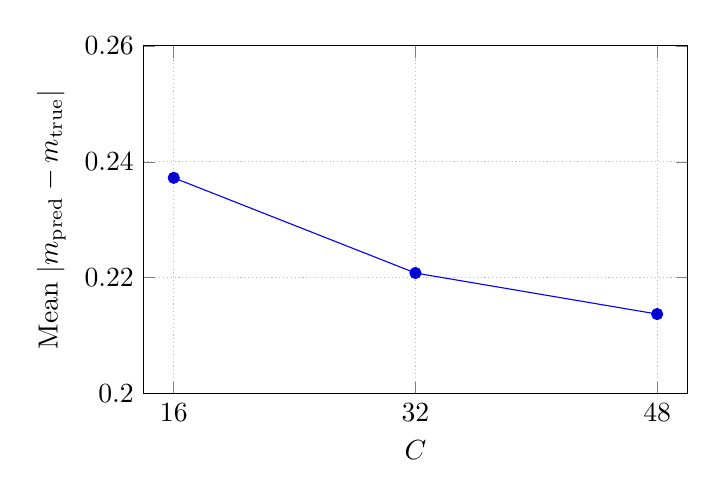
\begin{tikzpicture}
\begin{axis}[
  width=0.7\linewidth, height=6cm,
  xlabel={$C$}, ylabel={Mean $|m_{\rm pred}-m_{\rm true}|$},
  ymin=0.20, ymax=0.26, xmin=14, xmax=50,
  xtick={16,32,48}, ytick={0.20,0.22,0.24,0.26},
  grid=both, grid style={densely dotted}
]
\addplot coordinates {(16,0.237235) (32,0.220815) (48,0.213736)};
\end{axis}
\end{tikzpicture}
\caption{Mean absolute error decreases as $C$ grows (fixed $A=2.5$; $j\le 50$).}
\end{figure}

\noindent\textit{Data files.}
Complete \(j=1..50\) tables (predicted vs.\ true) for \((A,C)=(2.5,32)\) and \((2.5,48)\) are available in a companion repository (anonymized for review) and on request; filenames: %% [PATCH P4]
\begin{itemize}[leftmargin=1.2em]
\item \texttt{m\_pred\_vs\_truth\_j1\_50\_A2p5\_C32\_float.csv}
\item \texttt{m\_pred\_vs\_truth\_j1\_50\_A2p5\_C48\_float.csv}
\end{itemize}
(These can be typeset as a \texttt{longtable} if desired; we omit the 50-line listings here to conserve space.)

\bigskip
% >>> NEW: RH-dependency ledger box (explicit)
\begin{center}
\fbox{\begin{minipage}{0.94\linewidth}
\textbf{RH–dependency ledger (Part~III).}
\begin{itemize}
\item \emph{RH–free:} algebra on the parity lattice; Cor.~\ref{cor:canonical-columns}--\ref{cor:curvature}; pinning (Cor.~\ref{cor:pinning}); robustness (Lemma~\ref{lem:robust}); existence/uniqueness/contraction of the deterministic generator (Thm.~\ref{thm:generator}); argument–principle tie‑in (Prop.~\ref{prop:AP-tiein}) as a counting statement.
\item \emph{Uses columns collapse (RH in width–2):} Identifying the amplitude $\Imag d(2j{-}1)$ with the \emph{complete} set of ordinates $t_j$ so that $u=1+i\,m_j$ exhausts all nontrivial zeros.
\end{itemize}
\end{minipage}}
\end{center}

%------------------------------------------------------------------------------------------
% Appendices
%------------------------------------------------------------------------------------------

\appendix

\section{Hinge--Unitarity: a short proof}\label{app:hinge-short}
One may verify the monotonicity of \(\log|\chi_2|\) via \(\partial_\sigma\log|\Gamma|=\Real\psi\) and \(\psi(1-z)-\psi(z)=\pi\cot(\pi z)\); this yields the form recorded in Theorem~\ref{thm:hinge}.

\section{Constants ledger (sources \& transport)}\label{app:S2}
\begin{itemize}[leftmargin=1.2em]
\item Digamma (DLMF §5.11): \(\psi(z)=\log z+O(1)\) uniformly on vertical strips; transported to width–2 gives \(\Real\psi((1+v)/4)=\log|m|+O(1)\) on \(\partial B\).
\item \(\zeta'/\zeta\) (Titchmarsh §14; Ivi\'c Ch.~9): for \(1/2\le \sigma\le 1,\ t\ge 3\),
\(\displaystyle \frac{\zeta'}{\zeta}(\sigma+it)=\sum_{|\Imag\rho-t|\le 1}\frac{1}{\sigma+it-\rho}+O(\log t)\).
Removing local poles via \(\Zloc\) yields Lemma~\ref{lem:residual}.
\item Lipschitz Hilbert/Cauchy: bounded on \(L^2(\Gamma)\) for Lipschitz curves; boundary traces between \(\partial\D\) and \(\Gamma\) are bounded with constants depending only on the Lipschitz character (Coifman--McIntosh--Meyer).
\end{itemize}

\section{Bridges (one–liners)}
\begin{itemize}[leftmargin=1.2em]
\item Bridge~1. If \eqref{eq:rouche-ratio} holds, then \(E\) and \(\Gout\) have the same zero count, \(\Gout\) is zero‑free, \(|W|=1\) on \(\partial B\). Hence \(\log|W|\equiv 0\), and by open mapping \(W\equiv e^{i\theta_B}\).
\item Bridge~2. If \(W_1,W_2\) are unimodular constants on overlapping boxes, they agree on overlaps, hence globally.
\end{itemize}

\section{Conformal normalization}
Take \(\varphi:\D\to B(\alpha,m,\delta)\) conformal with \(\varphi(0)=\alpha+i m\) and \(\varphi(\pm 1)\) the top corners. By symmetry, \(\varphi((-1,1))\) is the horizontal centerline; thus there exists a unique \(r_0\in(0,1)\) with \(\varphi(\pm r_0)=\pm(a+im)\).

\section{Corner interpolation (detail)}
Rectangles are Wiener‑regular; continuous boundary data admit harmonic extension continuous up to \(\overline B\) (Kellogg; Axler--Bourdon--Ramey). Since \(h=0\) on arcs about \(C_\pm\), \(U=\log|G|\) there; exponentiating gives the corner modulus equality. Conformal boundary traces for polygons are classical (Ahlfors; Pommerenke).

\section{Outer/Rouch\'e certification protocol (rigorous outline)}\label{app:cert}
\begin{itemize}[leftmargin=1.2em]
\item Boundary intervals. Interval bounds for \(|E|\), \(\arg E\) on \(\partial B\).
\item Validated Poisson. Interval Dirichlet solver on \(\D\) for \(U=\log|\,\Gout|\), with conformal push‑forward to \(\partial B\).
\item Phase reconstruction. Interval Hilbert on \(\partial\D\), conformal trace to \(\partial B\).
\item Grid\(\to\)continuum. Lipschitz enclosure via \(\sup_{\partial B}|E'/E|\) and explicit pair terms.
\item Certificate. Check \(\sup_{\partial B}|E-\Gout|/|\,\Gout|<1\).
\end{itemize}

\section{Certified first nontrivial zero}\label{app:firstheight-certified}
We cite rigorously verified computations of Platt (and Platt--Trudgian):
\begin{theorem}[Platt 2017; Platt--Trudgian 2021]
There are no nontrivial zeros of $\zeta(s)$ with $0<\Imag s<t_1$, and the first nontrivial zero occurs at
$t_1=14.134725141734693790457251983562\ldots$ (with rigorous interval bounds).
\end{theorem}
References:
D.\,J.\,Platt, \emph{Isolating some nontrivial zeros of $\zeta(s)$}, Math. Comp. 86 (2017), 2449–2467;
D.\,J.\,Platt \& T.\,S.\,Trudgian, \emph{The Riemann hypothesis is true up to $3\cdot 10^{12}$}, Bull. Lond. Math. Soc. 53 (2021), 792–797.
Set $m_1:=2t_1$.

\section*{Appendix S.1. Operator norms on Lipschitz boundaries (shape-only dependence)}\label{app:S1}
On a Lipschitz Jordan curve \(\Gamma\) (e.g., the rectangle boundary), the boundary Hilbert transform is bounded on \(L^2(\Gamma)\) with norm depending only on the Lipschitz character; so is the Cauchy transform. Conformal boundary traces between \(\partial\D\) and \(\Gamma\) are bounded in \(L^2\) with operator norms depending only on chord–arc constants (Coifman--McIntosh--Meyer; Duren; Garnett). Since \(B(\alpha,m,\delta)\) normalizes affinely to a fixed square, all such operator norms are \emph{shape‑only}. We fold these into \(C_{\rm tr}\) (trace) and \(C_{\mathrm H}\) (boundary Hilbert norm) used in Lemma~\ref{lem:upper-disc}.

\section*{Appendix S.2. Instantiating $(C_1,C_2)$ from explicit literature bounds (optional)}\label{app:S2-nums}
Let \(F=E/Z_{\rm loc}\) with \(Z_{\rm loc}\) removing local zeros with \(|\Imag\rho-m|\le 1\). On \(1/2\le\sigma\le 1\) and \(t\ge 3\),
\[
\frac{\zeta'}{\zeta}(\sigma+it)=\sum_{|\Imag\rho-t|\le 1}\frac{1}{\sigma+it-\rho}+O(\log t)
\]
(Titchmarsh §14; Ivi\'c Ch.~9), and on vertical strips \(\psi\) satisfies \(\Real\psi(x+iy)=\log\sqrt{x^2+y^2}+O(1)\) (DLMF §5.11). Transporting to width~2 and dividing out \(Z_{\rm loc}\) yields
\(\sup_{\partial B}\big|{F'}/{F}\big|\ \le\ C_1\log m + C_2\)
with absolute constants \(C_1,C_2>0\). On \(\partial B\),
\(\frac{E'}{E}=\frac{F'}{F}+\frac{(Z_{\rm loc})'}{Z_{\rm loc}}\) (Lemma~\ref{lem:bridge-logs}); the local sum is finite by the boundary‑contact convention.

\section*{Appendix S.3. Pinned constants closing the band}\label{app:S3}
Choose
\[
\eta=10^{-3},\quad C_1=C_2=10,\quad C_{\mathrm{up}}=750,\quad C_h''=10,\quad K_{\rm alloc}^{\star}(\tfrac12)=3+8\sqrt{3}.
\]
At \(m=m_1=2t_1\) (Appendix~\ref{app:firstheight-certified}), worst case \(\alpha=1\), one has \(\delta=\eta/(\log m_1)^2\approx 8.96\cdot 10^{-5}\).
Then the upper bound \(\mathcal U_{hm}\le 2C_{\mathrm{up}}\,\delta^{3/2}(C_1\log m_1+C_2)\approx 0.0552\), while
\[
\mathcal L(m_1,1)=c_0\frac{\pi}{2}-\delta\Big(K_{\rm alloc}^{\star}(\tfrac12)\,c_0\,(C_1\log m_1+C_2)+C_h''(\log m_1+1)\Big)\approx 0.1206,
\]
so \(\mathcal U_{hm}<\mathcal L\). Monotonicity in \(m\) (LHS \(=o(1)\), RHS \(\to c_0\pi/2>0\)) then yields \(M_0(\eta)\le m_1\). No certified finite band is needed.

\section*{Appendix PW. A concrete Paley--Wiener weight}\label{app:PW}
Let \(\eta_0(y)=\exp(-1/(y(1-y)))\) on \(y\in(0,1)\) and 0 elsewhere. Set \(c_W:=\big(\int_0^1 \eta_0(y)\,dy\big)^{-1}\) and \(W(y):=c_W\,\eta_0(y)\).
Then \(W\in C_c^\infty([0,1])\), \(W\ge0\), \(\int_0^1W=1\), and \(\sup W=:C_W<\infty\) (note \(C_W>1\) for this normalization; the bound \(0\le W\le1\) is \emph{not} required anywhere).
With this \(W\):
\begin{itemize}[leftmargin=1.2em]
\item (Chebyshev--type bound) \(\sum_{n\le X}\Lambda(n)/\sqrt{n}\cdot W(n/X)\ \ll\ \sqrt{X}\).
\item (Cubic sinusoid remainder) The cubic remainder in Cor.~\ref{cor:C2} is \(\ll (\log X)^2\sqrt{X}/(\log m)^3\).
\end{itemize}

% -----------------------------------------------------------------------------------------
% Bibliography
% -----------------------------------------------------------------------------------------

\clearpage
\addcontentsline{toc}{section}{References}
\begin{thebibliography}{99}

\bibitem{Ahlfors}
L.~V.~Ahlfors, \emph{Complex Analysis}, 3rd ed., McGraw--Hill, 1979.

\bibitem{AxlerBourdonRamey}
S.~Axler, P.~Bourdon, and W.~Ramey, \emph{Harmonic Function Theory}, 2nd ed., Springer, 2001.

\bibitem{CoifmanMcIntoshMeyer}
R.~R.~Coifman, A.~McIntosh, and Y.~Meyer,
L’int\'egrale de Cauchy d\'efinit un op\'erateur born\'e sur $L^2$ pour les courbes lipschitziennes,
\emph{Ann. of Math.} \textbf{116} (1982), 361--387.

\bibitem{Conway}
J.~B.~Conway, \emph{Functions of One Complex Variable}, 2nd ed., Springer, 1978.

\bibitem{DLMF}
NIST Digital Library of Mathematical Functions, \S5.5 (Digamma reflection), \S5.11 (vertical--strip bounds).
\url{https://dlmf.nist.gov/}

\bibitem{DurenHp}
P.~L.~Duren, \emph{Theory of $H^p$ Spaces}, Academic Press, 1970.

\bibitem{GarnettBAF}
J.~B.~Garnett, \emph{Bounded Analytic Functions}, Springer, 2007.

\bibitem{GarnettMarshall}
J.~B.~Garnett and D.~E.~Marshall, \emph{Harmonic Measure}, Cambridge Univ. Press, 2005.

\bibitem{Ivic}
A.~Ivi\'c, \emph{The Riemann Zeta-Function}, John Wiley \& Sons, 1985.

\bibitem{Kellogg}
O.~D.~Kellogg, \emph{Foundations of Potential Theory}, Dover, 1953.

\bibitem{Platt2017}
D.~J.~Platt, Isolating some nontrivial zeros of $\zeta(s)$, \emph{Math. Comp.} \textbf{86} (2017), 2449–2467.

\bibitem{PlattTrudgian2021}
D.~J.\,Platt and T.\,S.~Trudgian, The Riemann hypothesis is true up to $3\cdot 10^{12}$,
\emph{Bull. Lond. Math. Soc.} \textbf{53} (2021), 792–797.

\bibitem{Pommerenke}
Ch.~Pommerenke, \emph{Boundary Behaviour of Conformal Maps}, Springer, 1992.

\bibitem{Ransford}
T.~Ransford, \emph{Potential Theory in the Complex Plane}, Cambridge Univ. Press, 1995.

\bibitem{Titchmarsh}
E.~C.~Titchmarsh (rev. D.~R.~Heath--Brown), \emph{The Theory of the Riemann Zeta-Function}, 2nd ed., Oxford, 1986.

% >>> NEW: dataset citation for numerical ordinates (first 50)
\bibitem{LMFDB}
The LMFDB Collaboration, \emph{The L-functions and Modular Forms Database},\\
Zeros of the Riemann zeta function (download interface for initial ordinates).

\end{thebibliography}

\clearpage
\section*{Authorship and AI--Use Disclosure}
\addcontentsline{toc}{section}{Authorship and AI--Use Disclosure}
The author, Dylan Anthony Dupont, designed the framework, chose constants/normalizations, and validated all mathematics and computations. Generative assistants (from GPT–4o to GPT–5 Pro) were used for typesetting assistance, editorial organization, and consistency checks, and are not authors. All claims are the author's responsibility.

\end{document}
